\documentclass[a4paper,10pt]{report}

\usepackage[in]{fullpage}
\usepackage{parskip}
\usepackage{hyperref}
\usepackage{tikz}
\usepackage{amsmath}
\usepackage[backend=bibtex,style=numeric-comp,sorting=nyt,sortcites=true,maxnames=4]{biblatex}
\usepackage[section]{placeins}
\usepackage[color]{circus}
\usepackage{fixltx2e}

\title{Qualifying Dissertation}
\author{James Baxter}
\date{}

\bibliography{literature} 

%TC:group zed 0 displaymath
%TC:group axdef 0 displaymath
%TC:group schema 1 displaymath
%TC:group circus 0 displaymath
%TC:group circusaction 0 displaymath
%TC:macroword \Circus 1 

\begin{document}
\maketitle

\begin{abstract}
  In recent years Java has been increasingly considered as a language for
  safety-critical embedded systems.  However, some features of Java are
  unsuitable for such systems and this has resulted in the creation of
  Safety-Critical Java (SCJ).  The different scheduling and memory management
  model of SCJ means that a specialised virtual machine is required to run SCJ
  programs.  Given the safety-critical nature of the applications, it must be
  ensured that the virtual machine is correct, but so far no SCJ vitual machine
  has been formally verified.  In this dissertation, we propose a framework for
  verification of SCJ virtual machines.  We consider the differences between SCJ
  and standard Java, and discuss some of the existing virtual machines for SCJ.
  Seeing that many SCJ virtual machines precompile to native code, we then
  survey some of the literature on compiler correctness.  Finally, we present
  some preliminary results identifying the requirements of the services of an
  SCJ virtual machine and constructing a formal model of those requirements.
\end{abstract}

\tableofcontents

\chapter{Introduction}

This chapter begins by explaining the motivation for the work described in this
dissertation. Afterwards, the objectives of the work, which come from the
motivation, are described and, finally, the structure of the remainder of this
dissertation is described.

\section{Motivation}

Since its release in 1995, the Java programming language~\cite{gosling2013} has
increased in popularity and is now in use on many platforms.  This popularity
means that Java has been used in a wide variety of areas including desktop
applications, on the internet in the form of Java applets, on
smartcards~\cite{chen2000} and on mobile devices~\cite{oracle2014}.  Several
languages derived from Java have also been created, including
Scala~\cite{lausanne2015} and Ceylon~\cite{redhat2015}, as well as older
variants of Java such as MultiJava~\cite{clifton2006} and
Pizza~\cite{odersky1997}, which have in turn contributed to the development of
Java. Scala adds functional programming features to Java, some of which have
been incorporated into Java 8. Ceylon extends Java's type system with features
such as union types, allowing some common Java errors to be checked at compile
time through the type system.

One use of Java that is of particular interest is in embedded systems.  While
early versions of Java were developed for programming, particularly TV set-top
boxes, the technology was not well received. It was only in the growing sector
of the internet that Java initially found a market~\cite{horstmann2002}.
However, it was soon realised that the portability, modularity, safety and
security benefits of Java could be of great use in embedded
systems~\cite{mulchandani1998}.  This required the creation of specialised Java
virtual machines as the standard JVM is too large for most embedded systems.
Much research has gone into making increasingly smaller virtual machines to
widen the range of devices that Java can be used on~\cite{caska2011,thomm2010}.

Many embedded systems are also real-time systems, and features of Java such as
the garbage collector and the concurrency model make it unsuitable for real-time
systems, for which strict guarantees about timing properties must be made.  To
address this issue the Real-Time Specification for Java
(RTSJ)~\cite{gosling2000} was created.  The RTSJ extends Java with a scoped
memory model and a more predictable scheduling system.

While the RTSJ addresses real-time requirements of embedded systems, many
embedded systems are also safety-critical.  For these conformance to certain
standards, such as \mbox{DO-178C} and ISO~26262, is required.  To support the
development of safety-critical programs that meet these requirements in Java,
the Safety-Critical Java (SCJ) specification~\cite{locke2013} has been created.
SCJ is a subset of the RTSJ that removes the features that cannot be easily
statically reasoned about, which means that features such as the
garbage-collected heap and dynamic class loading are absent from SCJ.  This
facilitates the creation of SCJ programs that fulfil formal specifications;
indeed work has already been done on developing correct SCJ programs from formal
specifications~\cite{cavalcanti2011, cavalcanti2013}.

On the other hand, even if it can be shown that SCJ programs are correct, it
must still be ensured those programs are executed correctly.  In the case of
Java-like languages, this generally means ensuring the Java compiler and Java
Virtual Machine (JVM) are correct.

Work has been done on modelling virtual machines for Java, and on the formal
correctness of compilers targeting those virtual machines.  Some of the most
complete work in that area was by St\"{a}rk, Schmid and
B\"{o}rger~\cite{stark2001}, who present a model of the full Java language and
virtual machine, along with a formally verified compiler, although for an older
version of Java than is current.  Other work has also been done on modelling the
JVM and Java compilation using refinement
techniques~\cite{duran2010}. Additionally there has been work considering
machine checked models of Java virtual machines and
compilers~\cite{lochbihler2012, nipkow2000, strecker2002}. Work has also been
done on the semantics of Java bytecode and verification of standard
JVMs~\cite{bertelsen2000, jones1998}.

However, SCJ has a number of differences from standard Java. Firstly, as already
indicated the SCJ memory model is rather different to the standard Java memory
model, abandoning the garbage collector in favour of a scoped memory model.
Garbage collection is less predictable and often quite complex, and so difficult
to reason about and unsuitable for some of the strictest certifiability
requirements of safety-critical systems.  By contrast, the scoped memory model
provides greater predictability on when memory is freed.  Similarly, the SCJ
approach to scheduling differs from that of standard Java, using a preemptive
priority scheduling approach rather than the unpredictable scheduling of
standard Java threads.  These differences of SCJ from standard Java mean that
the standard JVM is not suitable for running SCJ programs.  A specialised
virtual machine is required.

In the case of virtual machines for embedded systems, the priorities are usually
size and speed, which generally results in machines that are hard to verify.
Moreover, virtual machines that rely on interpreting bytecode are unsuitable for
real-time embedded systems as they are likely to be slower.  An alternative
method to run a Java program is to compile it to native code and some authors
have suggested doing so either directly~\cite{schultz2003} or via
C~\cite{varma2004}. There are several virtual machines that take this approach
including Fiji VM~\cite{pizlo2009}, Icecap HVM~\cite{sondergaard2012} and
OVM~\cite{armbruster2007}.  This allows correct running of an otherwise correct
SCJ program to be viewed as a compiler verification problem.

There has been much research into compiler correctness.  Much of the work
follows a commuting diagram approach, in which the compilation is shown to be
consistent with transformation between the semantics of the source and target
languages\cite{morris1973, thatcher1979}. This approach is apparent in much of
the early work such as that of McCarthy and Painter~\cite{mccarthy1967}, as well
as in more recent work such as the CompCert project~\cite{leroy2009a,
  leroy2009b}. There has also been work that follows this approach and employs
automated theorem provers~\cite{klein2006, milner1972, nipkow2000}. They provide
additional certainty that the proof is correct and can also provide code
generation facilities to allow creation of a working compiler.

An alternative is the algebraic approach to compiler
verification~\cite{hoare1991, sampaio1993}, based on modelling compilation using
refinement calculi~\cite{back1981, morgan1990, morris1987}. This approach
appears to be less commonly used but has been applied to Java~\cite{duran2005,
  duran2010} and hardware description languages~\cite{perna2010,
  perna2011}. This approach is also quite amenable to automation as it relies on
refinement laws that can be applied by a term rewriting system.

There is a clear need for formal verification of SCJ virtual machines due to the
safety-critical nature of the systems involved and the fact that safety
standards such as DO-178C require it at the highest safety levels. However,
there appears to be little work done in that area and, as far as we know, no SCJ
virtual machine has been formally verified.

% explain that there is a gap with no verification for SCJ compilers for embedded systems

\section{Objectives}

Our objective is to construct a framework for verification of an SCJ virtual
machine.  It will provide the following resources for developers and verifiers:
\begin{itemize}
\item a specification of the requirements of an SCJ virtual machine,
\item a compilation strategy from Java bytecode to native C code,
\item a formal model of the virtual machine specification,
\item proofs for validation of the formal model and verification of the
  compilation strategy, and
\item a mechanisation of the model and proofs.
\end{itemize}

The first component required is a specification of the requirements for an SCJ
virtual machine. This specification will shape the rest of the work and there is
at present no clear specification of what is required of an SCJ virtual machine
or how it differs from a standard Java virtual machine.  The specification of
requirements needs to consider the requirements imposed, both explicitly and
implicitly, on virtual machines by the SCJ specification~\cite{locke2013} as
that provides the authoritative source for information on SCJ.  It is also
helpful to consider the approach taken by some existing SCJ virtual machines on
points where the SCJ specification is unclear.  The virtual machine must also
meet the standard Java Virtual Machine specification~\cite{lindholm2014} on
points such as how to interpret Java bytecode instructions.  There is much work
on the semantics of Java bytecode that can be leveraged in our
work~\cite{bertelsen2000, jones1998, stark2001}.

As many existing virtual machines for SCJ precompile programs to native code in
order to allow faster execution on embedded systems, it seems wise to include
that in our framework.  We will focus on compilation of Java bytecode to C as
that is the approach adopted by several existing virtual machines for embedded
systems, including Fiji VM~\cite{pizlo2009} and icecap
HVM~\cite{sondergaard2012}, and C is already widely used for embedded systems
software.

There are two main approaches to the specification and verification of
compilers: the commuting diagram approach and the algebraic approach.  The
commuting diagram approach involves specifying the compiler as a function from
the source language to the target language and showing that it is consistent
with transformation between the semantics of the source and target
languages~\cite{morris1973, thatcher1979}.  This approach has been used in much
of the work on compiler correctness, including some of the earliest
work~\cite{mccarthy1967} and recent work such as that of the CompCert
project~\cite{leroy2009a, leroy2009b}.

The algebraic approach involves defining the source and target languages in the
same specification space, and using proved specialised rewrite rules to
characterise compilation as model transformation in the extended language. This
approach was first proposed in the early nineties by Hoare~\cite{hoare1991} and
further developed by Sampaio~\cite{hoare1993, sampaio1993}.  The algebraic
approach does not seem to be as popular as the commuting diagram approach, but
it does have the advantage that the specification of the compilation strategy is
correct by construction as the rewrite rules that comprise it have all been
proved.

In order to ensure that the specification is precise and to facilitate proofs of
its correctness, it must have a model written in some formal specification
language.  We will focus on using the \Circus{} specification
language~\cite{oliveira2009}, as it has been used in some of the previous work
on formalising SCJ~\cite{cavalcanti2011, cavalcanti2013}.  It is important that
the correctness of the formal models and compilation strategy can be shown via
mathematical proof, which requires the specification language to have a
well-defined semantics.  \Circus{} has such a semantics, defined using the model
of Unifying Theories of Programming (UTP)~\cite{hoare1998}.

To prevent mistakes in the proofs, it is helpful to mechanise the formal model
and proofs.  There are various systems that can be used for this, but we will
focus on the proof assistant Isabelle~\cite{nipkow2002, nipkow2014}. It has
existing mechanisations of \Circus{}~\cite{feliachi2012} and the
UTP~\cite{foster2015}, and has been used in previous work verifying compilers
for Java-like languages~\cite{klein2006, strecker2002, lochbihler2010}, making
it well placed for our work.

We have already made some progress towards the construction of the proposed
framework with a specification and formal model of the requirements of an SCJ
virtual machine.  It is expected that the model will be checked using a theorem
prover; our next task is then the development of a compilation strategy to
native code.

\section{Document Structure}

Having given a brief overview of the area of study and identified the problem we
wish to consider, the remainder of this dissertation proceeds as follows.

In Chapter~\ref{literature-review-chapter} we examine the literature on
safety-critical virtual machines and compilers for Java-like languages. This
includes a discussion of why a safety-critical variant of Java is necessary and
how it differs from standard Java.  We also explain why a specialised virtual
machine is necessary for SCJ.  This is followed by a survey of the existing
virtual machines for Safety-Critical Java and the techniques used in verifying
compilers.

In Chapter~\ref{research-proposal-chapter} we will cover the structure and
plan for the proposed research.

In Chapter~\ref{requirements-chapter} we present some preliminary results
identifying the requirements of an SCJ virtual machine, with a formal model of
those requirements in the \Circus{} specification language.

Finally, we conclude in Chapter~\ref{conclusions-chapter} by summarising our
contributions and mentioning the wider context of this research.

% Description of SCJ and review of SCJ VMs - use stuff from JTRES paper, maybe extend it a bit
% Review the literature on compiler correctness 
%  - Two approaches: algebraic and commuting diagram
%  - Consider each approach in a separate subsection and compare them
%  - Make sure to describe the *approach* in detail, not what the authors did
%  - Finish by looking at and comparing some of the work on Java compilation
% Present research proposal and preliminary results
% - Overall plan - requirements for an SCJVM - explain different parts of the diagram, mention CEE will be dealt with by later work
% - Present the identification of the requirements for the VM services from the JTRES paper
% - Discuss the formal model - similar to JTRES paper but room to go into more depth


\chapter{Compilers and Virtual Machines for Java-like languages in the Safety-critical Domain}
\label{literature-review-chapter}

This chapter begins with a discussion of why Java is being used in
safety-critical systems and the need for a specialised version of Java for use
in that area.  Then, in Section~\ref{scj-section} we cover the variant of Java
developed for safety-critical systems, how it differs from standard Java and why
a specialised virtual machine is required, before discussing some of the
existing virtual machines for that variant in
Section~\ref{virtual-machines-section}.

In Section~\ref{compiler-correctness-section} we survey some of the literature
on compiler correctness, and discuss the two main approaches in
Sections~\ref{commuting-diagram-subsection} and
\ref{algebraic-approach-subsection}, before seeing how the techniques of compiler
correctness have been applied to Java-like languages in
Section~\ref{java-compiler-correctness-subsection}.

In Section~\ref{circus-section}, we give an overview of the \Circus{}
specification language used for our virtual machine specification, before
concluding in Section~\ref{final-considerations-section}.

\section{Java for Safety-critical systems}
\label{java-safety-critical-section}

% provide motivation for SCJ, mentioning standard Java and RTSJ

In recent years Java has increasingly been considered as a language for writing
safety-critical software. Other languages that are generally used in the
safety-critical domain are C/C++ and Ada; C and C++ impose challenges concerning
reliable use at the highest levels of safety~\cite{kornecki2009}, and the
number of Ada programmers is not very large~\cite{bissyande2013}.  While Java has not
traditionally been seen as a language for safety-critical systems, it was
originally developed for the area of embedded systems, particularly for use in
television set-top boxes, and has seen renewed interest in its use in embedded
systems after gaining popularity in programming for the
internet~\cite{mulchandani1998}.

There are, however, several issues with standard Java that make it unsuitable
for safety-critical systems. Many safety critical systems are also real-time
systems, which are required to be predictable in their scheduling and use of
memory. However, standard Java uses a garbage-collected memory model, which
makes it hard to predict when memory may be freed or how long the process of
freeing memory may take. Standard Java's thread model also lacks the
predictability and control that is required in real-time systems.

To rectify these problems the Real-Time Specification for Java
(RTSJ)~\cite{gosling2000} was created; it augments Java's memory and scheduling
models with a system of scoped memory areas and a preemptive priority
scheduler. RTSJ also allows for the standard Java models to be used alongside
its own, making it suitable for a wide range of different real-time
applications.  On the other hand, this makes it hard to certify RTSJ
applications and thus renders the RTSJ unsuitable for use in the safety-critical
domain.

In order to allow certifiable safety-critical systems in Java, the
Safety-Critical Java (SCJ)~\cite{locke2013} specification was developed. SCJ is
a subset of the RTSJ that leaves out the features from standard Java that are
difficult to certify such as the garbage collector. SCJ also provides
annotations that allow memory usage to be more easily checked. We discuss SCJ in
more detail in the next section.

\section{Safety-Critical Java}
\label{scj-section}

SCJ removes the aspects of the RTSJ that make certification difficult, including
standard Java threads and the garbage collector.  This leaves scheduling and
memory management models that are very different to the models for standard Java
and that, therefore, require specialised virtual machines to support them.

SCJ defines three compliance levels to which programs and implementations may
conform. Level 0 is the simplest compliance level. It is intended for programs
following a cyclic executive approach. Level 1 lifts several of the restrictions
of level 0, allowing handlers that may trigger in response to external events
and preempt one another. Level 2 is the most complex compliance level, allowing
access to real-time threads and suspension via \texttt{wait()} and
\texttt{notify()}.  

An SCJ program consists of one or more missions, which are collections of
schedulable objects that are scheduled by SCJ's priority scheduler. Missions are
run in an order determined by a mission sequencer supplied by an SCJ program.
Running a mission proceeds in several phases, as shown in
Figure~\ref{phases-diagram}.

\begin{figure}[ht]
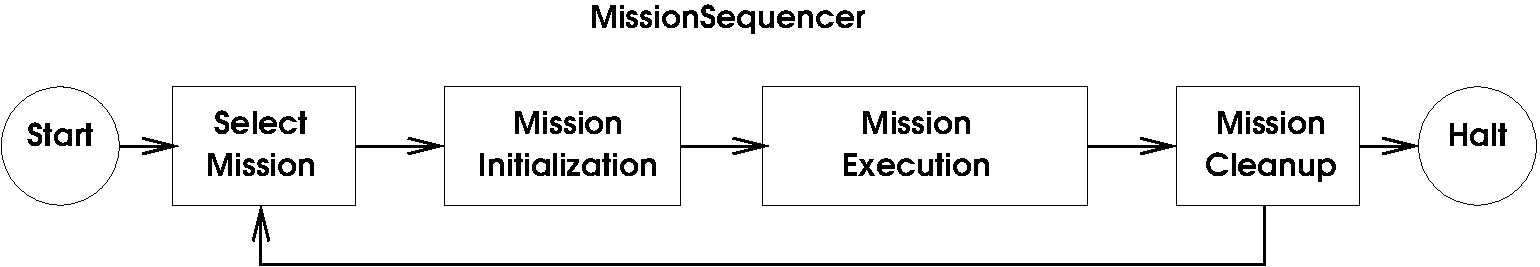
\includegraphics[width=\textwidth]{phases.pdf}
\caption{A diagram showing the phases of SCJ mission execution}
\label{phases-diagram}
\end{figure}

The fist phase is initialisation, which consists of setting up the schedulable
objects controlled by the mission and creating any data structures required for
the mission.  Then the mission is executed by starting each of the schedulable
objects in the mission and waiting for a request to terminate the mission. When
the mission is requested to terminate, each of the schedulable objects in the
mission is terminated and the mission's memory is cleared.

The schedulable objects within a mission are asynchronous event handlers that
are released either periodically, at set intervals of time, aperiodically, in
response to a release request, or once at a specific point in time (though
handlers that are released once can have a new release time set, allowing them
to be released again).  At level 2 real-time threads are also allowed, which run
continuously from when they start until they finish, unless they are suspended
or interrupted by another schedulable object.

Each schedulable object has a priority and the highest priority object that is
eligible to run at each point in time is the object that runs. This allows for
simpler reasoning about order of execution and allows for more urgent tasks to
preempt less urgent tasks.

SCJ allows for assigning schedulable objects to ``scheduling allocation
domains'', where each domain consists of one or more processors.  At Level 1,
each scheduling allocation domain is restricted to a single processor.  Hence,
in scheduling terms, the system is fully partitioned. This allows for mature
single processor schedulability analysis to be applied to each domain (although
the calculation of the blocking times when accessing global synchronised methods
are different than they would be on a single processor system due to the
potential for remote blocking~\cite{davis2011}).

SCJ deals with memory in terms of memory areas, which are Java objects that
provide an interface to blocks of physical memory called backing stores.  Memory
allocations in SCJ are performed in the backing store of the memory area
designated as the allocation context.  Each schedulable object has a memory area
associated with it that is used as the allocation context during a release of
that object, and is cleared after each release.  Each mission also has a mission
memory area that can be used as an allocation context by the schedulable objects
of that mission, to provide space for objects that need to persist for the
duration of the mission or to be shared between the schedulable objects.  There
is also an immortal memory area where objects can be allocated if needed for the
entire running of the program (they are never freed). SCJ places restrictions on
which objects an object may point to, so as to avoid dangling pointers from
being created. Some examples of valid and invalid object references for some
asynchronous event handlers are shown in Figure~\ref{stacks-areas-diagram}.

\begin{figure}[ht]
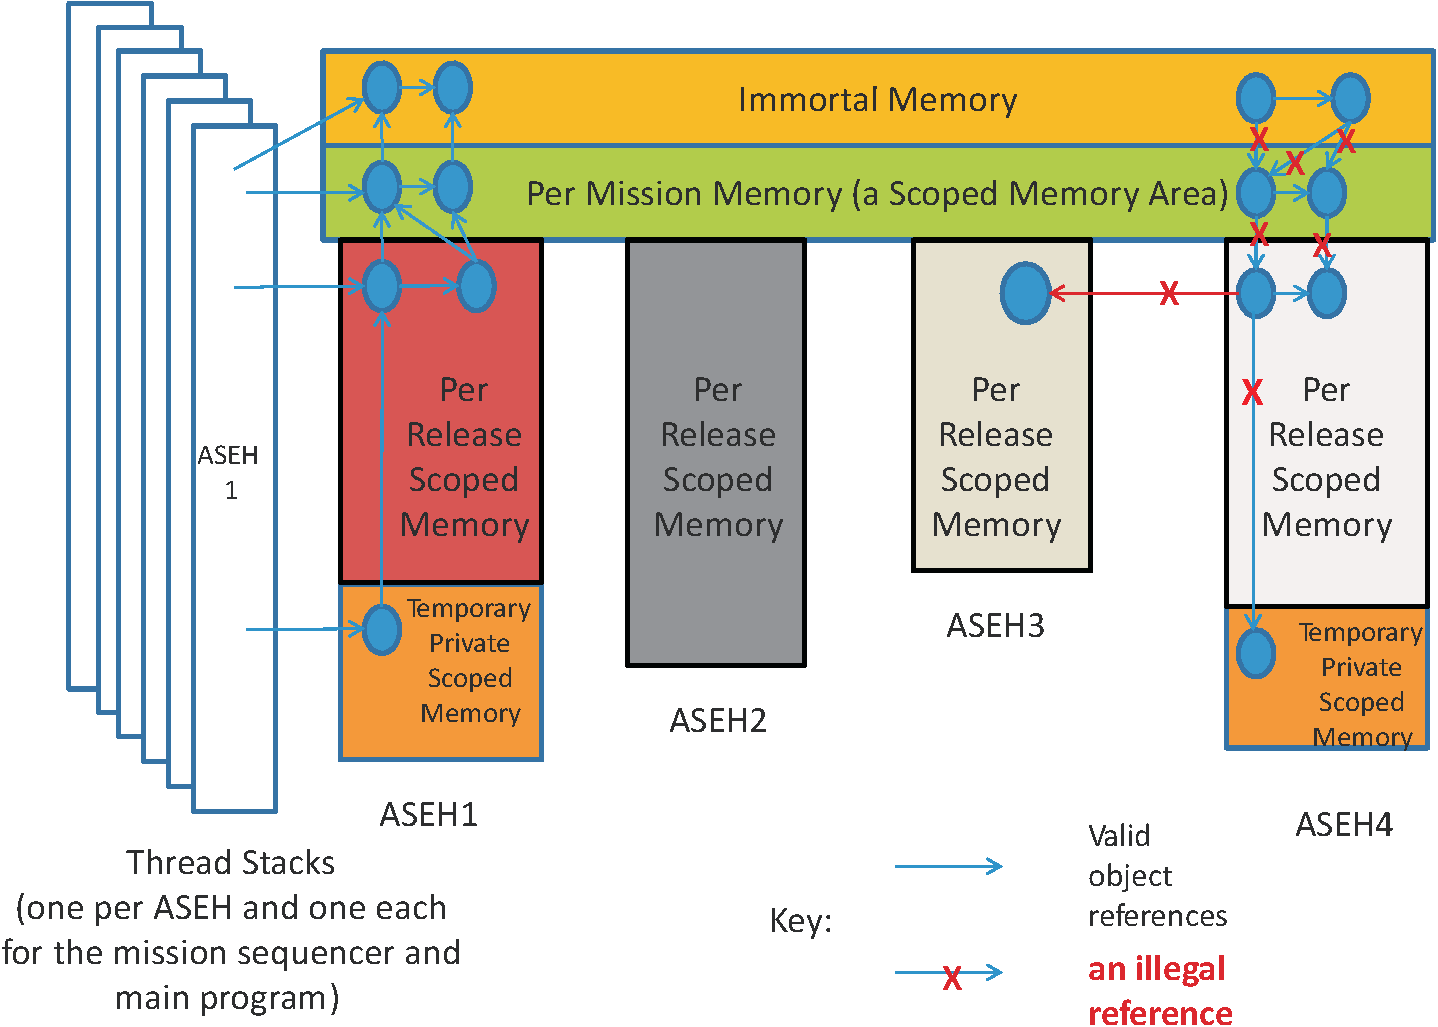
\includegraphics[width=\textwidth]{Stacks-Areas.pdf}
\caption{An example of the layout of memory areas for four asynchronous event
  handlers (ASEHs), showing possible valid and invalid references between them}
\label{stacks-areas-diagram}
\end{figure}

This system of memory areas makes it easy to predict when memory is freed.  It
is not supported by standard JVMs as they do not provide memory outside of the
heap for allocation and lack a notion of allocation context. The SCJ memory manager
also needs to provide a means of accessing raw memory for the purposes of device
access, but that section of the SCJ standard is not yet finalised so we will not
cover it here. It can, however, be seen that any system of raw memory access is
not supported by most standard JVMs.

Moreover, dynamic class loading is not allowed in SCJ; all classes used by the
program must be loaded when the program starts. This is because dynamic class
loading may introduce time overheads that are hard to predict and additional
code paths that complicate certification.  Finally, SCJ also disallows object
finalisers as it is not always easy to predict when they are run.

\section{Virtual Machines for Safety-Critical Java}
\label{virtual-machines-section}

% one subsection per machine

Because of the novel features of SCJ, briefly described in the
previous section, a specialised virtual machine that provides support
for allocation in memory areas and preemptive scheduling is required
for SCJ. Although SCJ is a relatively recent development there have
been various virtual machines created for SCJ or variations of SCJ,
including icecap HVM~\cite{sondergaard2012}, Fiji VM~\cite{pizlo2009},
OVM~\cite{armbruster2007}, HVM\textsubscript{TP}~\cite{luckow2014} and
PERC Pico~\cite{atego2015, richard2010}. These are each described in
the following subsections.

\subsection{icecap HVM and HVM\textsubscript{TP}}

The icecap hardware-near virtual machine (HVM) was created as part of the
Certifiable Java for Embedded Systems Project~\cite{schoeberl2014} and provides
an open-source implementation of SCJ targeted at embedded systems.  The
approach taken by the HVM is one of precompiling Java bytecode to C in order to
allow for faster running programs with fewer memory resources.  It includes an
implementation of the SCJ libraries that covers most of SCJ level 2, though only
for a single processor implementation.  This implementation, however, cannot be
easily decoupled from the virtual machine itself.

The icecap HVM also provides a lightweight Java bytecode interpreter and allows
for interpreted code to be mixed with compiled code.  The reason for this is
that the bytecode together with the interpreter can often be smaller than the
compiled code, though there is a tradeoff for speed. HVM\textsubscript{TP} is a
modification of the icecap HVM's bytecode interpreter to improve time
predictability and ensure that bytecode instructions are executed in constant
time, which is important for ensuring real-time properties of the system hold.

\subsection{Fiji VM}

Fiji VM is a proprietary Java implementation designed to run on real-time
embedded systems.  Similarly to the icecap HVM, Fiji VM uses the strategy of
compiling to C in order to improve performance.  However, Fiji VM is not
specifically targeted at SCJ and works with a range of libraries, including
SCJ, RTSJ and the standard Java libraries.  Fiji VM does have the advantage of
high portability and multiprocessor support, which is lacking in many other SCJ
virtual machines.

The fact that Fiji VM works with the SCJ libraries and supports the scoped
memory model means it can run SCJ programs.  It does not necessarily support all
aspects of SCJ properly though.

\subsection{OVM}

OVM was created at Purdue University as part of the PCES
project~\cite{baker2006}, to provide a virtual machine that can execute
real-time Java programs with a high level of performance on embedded systems.
Similar to Fiji VM and icecap HVM, OVM follows the principle of precompiling
code for performance reasons, but translates Java to C++ instead of bytecode to
C.

OVM also differs from the icecap HVM and Fiji VM in that it predates SCJ. It is
written to implement the RTSJ, though it can still support SCJ programs; indeed,
an SCJ implementation for OVM was later created~\cite{plsek2010}. However, OVM
does not appear to have kept up with more recent changes to the draft SCJ
standard. OVM is, like icecap HVM, but unlike Fiji VM, single processor.

\subsection{PERC Pico}

PERC Pico is a product of Atego based on early ideas for SCJ, but uses its own
system of Java metadata annotations to ensure the safety of scoped memory.  This
systems of annotations provides additional information about how memory is
used so that it can be checked.  Similarly to other SCJ virtual machines, PERC
Pico allows for precompilation of Java code but targets executable machine code
rather than an intermediate programming language.  The metadata annotations are
used to guide the compiler to produce code that uses the correct scoped memory.
PERC Pico does not support the current SCJ standard, though it has been
suggested that it could be modified to do so~\cite{nilsen2011}.

To summarise, as far as we are aware there is one publicly available virtual
machine that has kept up with the developing SCJ specification, the icecap
HVM. This is and, typically, virtual machines for SCJ will be, designed to be
very small and fast so as to be able to run on embedded systems.

As can be seen from the preceding discussion, a common technique to run Java
programs on embedded systems is to precompile them to native code. This means
compiler correctness techniques must be considered in verification of such a
virtual machine; these techniques are discussed in the next section.

\section{Compiler Correctness}
\label{compiler-correctness-section}

Due to the importance of compiler correctness, there has been much research over
the years in this area.  Most of the work done follows a similar approach, which
we will term the commuting-diagram approach as it is based on showing that a
particular diagram commutes. We will discuss the commuting diagram approach in
Section~\ref{commuting-diagram-subsection}.

An alternative approach to compiler verification is the algebraic approach
developed in the early 90s.  It is based on the concepts of refinement calculi
designed for deriving software from specifications of behaviour. We will explain
the algebraic approach in Section~\ref{algebraic-approach-subsection} and
discuss how it differs from the commuting-diagram approach.

We finish in Section~\ref{java-compiler-correctness-subsection} by reviewing
some of the literature on correctness of compilers for Java-like languages. We
explain how the techniques of compiler correctness have been applied in the case
of Java and compare the different approaches.

\subsection{Commuting-diagram Approach}
\label{commuting-diagram-subsection}

Much of the work on compiler correctness can be seen as following the approach
identified by Lockwood Morris~\cite{morris1973}, and later refined by Thatcher,
Wagner and Wright~\cite{thatcher1979}. The approach is essentially that a
compiler correctness proof is a proof that the diagram shown in
Figure~\ref{commuting-diagram} commutes, that is, $\gamma \circ \psi = \phi
\circ \epsilon$.

\begin{figure}[ht]
  \begin{center}
    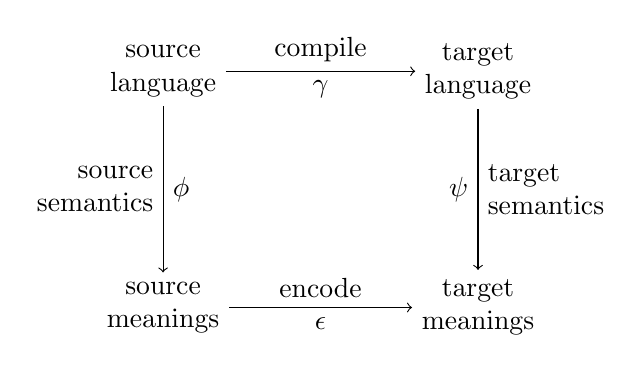
\begin{tikzpicture}
      \node[align=center] (S) at (0cm,3cm) {source\\language};
      \node[align=center] (T) at (4cm,3cm) {target\\language};
      \node[align=center] (M) at (0cm,0cm) {source\\meanings};
      \node[align=center] (U) at (4cm,0cm) {target\\meanings};
      
      \path (S) edge[->] node[align=center, above] {compile}           
        node[align=center, below] {$\gamma$} (T);
      \path (S) edge[->] node[align=right, left]   {source\\semantics} 
        node[align=center, right] {$\phi$} (M);
      \path (T) edge[->] node[align=left, right]   {target\\semantics} 
        node[align=center, left] {$\psi$} (U);
      \path (M) edge[->] node[align=center, above] {encode} 
        node[align=center, below] {$\epsilon$} (U);
    \end{tikzpicture}
  \end{center}
  \caption{The commuting diagram used in the traditional approach to compiler verification}
  \label{commuting-diagram}
\end{figure}

Lockwood Morris had the corners of the diagram as algebras, rather than merely
sets, with the functions between them being homomorphisms in order to add
additional structure to the proof.  This differs from the approach of some
earlier works, particularly the earliest work by McCarthy and
Painter~\cite{mccarthy1967}, and instead follows work such as that of Burstall
and Landin~\cite{burstall1969}.

McCarthy and Painter's work featured a simple expression language with addition,
natural numbers and variables.  This was compiled to a simple 4-instruction
single-register machine.  The arrows of the diagram were simple functions,
rather than homomorphisms, and the proof was performed using induction over the
source language. This work laid the foundation for the study of compiler
correctness.

Burstall and Landin show correctness of a compiler for the same source and
target languages as McCarthy and Painter; they use a more algebraic approach
that better matches what Lockwood Morris later suggested.  Burstall and Landin's
approach involved representing the source and target languages, and their
meanings, as algebras, with the compilation functions as homomorphisms. They
target several intermediate machines in the proof of correctness. Viewing the
languages as algebras allows for simpler proofs as some of the arrows of the
commuting diagram can be wholly or partially derived from the algebraic
structure. It was this goal of simplifying the proofs that led Lockwood Morris
to advocate the use of algebras and homomorphisms.

The overall goal of pursuing formal proofs of compiler correctness, as proposed
by McCarthy and Painter~\cite{mccarthy1967}, is to allow machine-checked proofs
of program correctness. There has been work in that area, the earliest of which
is that by Milner and Weyhrauch~\cite{milner1972} who show the correctness of an
ALGOL-like language. The proof of correctness was partially mechanised in the
LCF theorem prover~\cite{milner1972a} and the authors were of the opinion that
the proof was feasible and could be completed relatively easily. A point to note
is that Milner and Weyhrauch acknowledged the need for some way of structuring
the proof in order to make it amenable to machine-checking. This gives further
support to the algebraic commuting diagram approach advocated by Lockwood
Morris. Indeed, Milner and Weyhrauch explicitly followed that approach as they
were in discussions with Lockwood Morris.

One advantage to making proofs easily machine-checkable, apart from the added
certainty that the proof is correct, is that working compilers can be created
from the machine-checked proofs.  Code generation facilities are available with
many theorem provers such as those of Isabelle/HOL~\cite{haftmann2007} and
Coq~\cite{letouzey2003, letouzey2008}. The fact that the commuting-diagram
approach involves treating the compilation as a function between algebras
representing the source and target languages fits well with this idea. In this
case, there is then a function defined in the mechanised logic for the purposes
of conducting proofs about it that can be readily extracted to executable code.

The commuting-diagram approach has been followed in much of the literature
through the years, though not always with the algebraic methods recommended by
Lockwood Morris.  The basic structure of the commuting diagram is a fairly
natural approach to take, as seen by work such as that of the ProCoS
project~\cite{buth1992}.

Another piece of work that follows the commuting diagram approach is that of
Polak~\cite{polak1981}, who states that he is more interested in verification of
a ``real'' compiler rather than ``abstract code generating algorithms'', and
shows the correctness of a compiler for a Pascal-like language.  This work
focuses much more on pragmatic applications of the commuting-diagram approach,
leaving behind the algebraic ideas of earlier papers.  It sets a precedent for a
simpler verification approach based on considering the functions in the
commuting diagram.

The commuting diagram has also been used in recent work, some of the most
successful of which is that of CompCert~\cite{leroy2009a, leroy2009b,
  leroy2012}.  This is a project to create a fully verified realistic compiler
for a subset of C, using the theorem prover Coq~\cite{coq2004}.

\subsection{Algebraic Approach}
\label{algebraic-approach-subsection}

The second main approach to showing correctness of compilers is the
algebraic approach proposed by Hoare in 1991~\cite{hoare1991}, and
further developed by Sampaio~\cite{hoare1993, sampaio1993,
  sampaio1997}. We note that the algebraic approach discussed in this
section is largely unrelated to the algebraic commuting-diagram
approaches mentioned in the previous section.

The algebraic approach to compilation derives from the concepts of algebraic
reasoning about programs and program refinement. These concepts come from the
idea, proposed by Hoare in 1984~\cite{hoare1984}, that programs can be thought
of as predicates and so the laws of predicate logic can be used to construct
laws for reasoning about programs~\cite{hoare1987}. As an example of such a law
for reasoning about programs, we present below associativity of sequential
composition, Equation~\eqref{seq-comp-assoc}, and left and right unit of
sequential composition, namely, the program $\Skip$ that does nothing,
Equation~\eqref{skip-comp-identity}.
\begin{equation}
  \label{seq-comp-assoc}
  P;(Q;R) = (P;Q);R
\end{equation}
\begin{equation}
  \label{skip-comp-identity}
  P;\Skip = \Skip;P = P
\end{equation}

The notion of refinement is central to the algebraic approach to compilation.
Refinement calculi have been developed, independently, by Back~\cite{back1981},
Morris~\cite{morris1987} and Morgan~\cite{morgan1990}, following from earlier
concepts of program transformation~\cite{bauer1976, balzer1976, standish1976,
  arsac1979}.  The basic idea is that there is a relation between programs that
captures the idea of one program being ``at least as good as'' another or, to
put it more precisely, at least as deterministic as another.  Languages and laws
for reasoning about programs can also be used to develop programs from
specifications.  This means that certain aspects of a system can have a
nondeterministic specification and several different implementations can refine
that specification.

In using refinement in showing correctness of a compiler, the laws of the
specification language can be used to prove compilation refinement laws.
Compilation laws can be used to transform the source programs into some normal
form that represents an interpreter for the target language.  In other words,
the code output by the compiler, when executed by on the target machine, must be
a refinement of the source program.  The compilation laws can be used to prove
this refinement and at the same time generate the target code.

As an example, consider the following refinement in which a simple program that
performs some arithmetic and stores the results into variables is refined by a
normal form representing the target machine.  The symbol $\circrefines$
represents the refinement relation here.
\begin{equation}
\circvar x, y, z \circspot x := (x + 5) \times (y + z) ; z := z + 1
\circrefines
\begin{aligned}
&\circvar A, P, M \circspot P := 1; \circdo \\
&\quad            P=1  \then A,    P := M[2],          2 \\
&\quad \extchoice P=2  \then A,    P := A + M[3],      3 \\
&\quad \extchoice P=3  \then M[4], P := A,             4 \\
&\quad \extchoice P=4  \then A,    P := M[1],          5 \\
&\quad \extchoice P=5  \then A,    P := A + 5,         6 \\
&\quad \extchoice P=6  \then A,    P := A \times M[4], 7 \\
&\quad \extchoice P=7  \then M[1], P := A,             8 \\
&\quad \extchoice P=8  \then A,    P := M[3],          9 \\
&\quad \extchoice P=9  \then A,    P := A + 1,         10 \\
&\quad \extchoice P=10 \then M[3] := A,               11 \\
&\circod ; \{ P = 11 \}
\end{aligned}
\end{equation}
The normal form introduces 3 variables: $A$, which represents the a general-purpose
register of the target machine; $P$, which represents the program counter of the
target machine; and $M$, which is an array representing the memory of the target
machine.  The normal form consists of a program that initialises $P$ to 1 and
then enters a loop in which the operation performed on each iteration is
dependent on the value of $P$.  The loop is exited when $P$ is set to a value
for which there is no operation and it is asserted that $P$ will be equal to 11
at the end of the program.  Each of the statements of the source program
corresponds to several operations in the normal form as complex expressions are
broken down into simpler expressions that can be handled by instructions of the
target machine.  This process also introduces the register $A$ and a temporary
variable to store the intermediate results.  The temporary variable is what
appears in the normal form as $M[4]$.  This temporary variable, as well as the
variables $x$, $y$ and $z$ from the source program, get replaced with locations
in the memory array $M$ in a process called data refinement.  Each of the
assignment statements from breaking down the expressions is refined by a normal
form with an explicit program counter $P$.  These normal forms are then combined
to create the normal form of the full program.  The update of the program
counter in this program is quite simple but more complex updates would occur for
conditionals or loops.

The power of the algebraic approach is that the compilation of individual
elements of the source language can be specified and proved separately in
different refinement laws.  The compilation can also be split into stages, with
a set of refinement laws for each stage to modularise the compilation.  The
separate refinement laws can then be combined to form a compilation strategy.

The first major work done using the algebraic approach was that of
Sampaio~\cite{sampaio1993}, who used it to specify a correct compiler for a
simple language that, nonetheless, covers all the constructs available in most
programming languages. The target machine Sampaio used was a simple
single-register machine that bears similarity to most real processor
architectures.  He mechanised the compiler in the OBJ3 term rewriting
system~\cite{goguen1988}, showing that working compilers can be easily created
from specifications using the algebraic approach.  However, the algebraic laws
Sampaio used to prove correctness of the compiler were taken as axioms. Sampaio
notes that they could be easily proved given a semantics for the reasoning
language.

Though there has not been much work done using the algebraic approach, we single
out the work of Perna~\cite{perna2010, perna2011}, showing correctness of a
compiler for a hardware description language.  The compilation takes high-level
descriptions of hardware written in Handel-C and transforms them into systems of
basic hardware components connected by wires.  The algebraic approach works well
here as the target language is a subset of the source language, albeit in a
different form.  Perna was able to handle features not covered by most other
works on hardware compilation, such as parallelism with shared variables.  Also,
whereas Sampaio took the basic algebraic laws as axioms, Perna proved the laws
from a semantics given using the Unifying Theories of Programming (UTP)
model~\cite{hoare1998}.  There has also been work on the correctness of Java
compilers using the algebraic approach.  This is considered in the next section,
where we consider compiler correctness for Java-like languages.

\subsection{Correctness of Java Compilers}
\label{java-compiler-correctness-subsection}

The popularity of Java has meant that there has been plenty of work on
formalising Java and the JVM~\cite{hartel2001}, but there have been relatively
few works on formally verified compilers for Java-like languages.  However, the
work that has been done uses both of the two main approaches and covers most of
the features of Java.

Some of the earliest and most thorough work is that by S\"{a}rk, Schmid and
B\"{o}rger~\cite{stark2001}, who formalise most of Java and the JVM before
specifying and showing the correctness of a compiler for Java.  The approach
taken by them uses Abstract State Machines (ASMs) to specify the source and
target languages.  The ASMs give an operational semantics to Java and the JVM,
describing how each construct affects the running of the program.  The languages
are each specified by multiple ASMs, beginning with an imperative core, then
adding classes, objects, exceptions and, finally, threads.

Although this approach is called the ASM approach, it becomes clear from the
definition of compiler correctness given in terms of a mapping between ASMs that
this work ultimately follows the commuting-diagram approach.  This work leaves
parts of the proof incomplete (in particular, compilation of threads is not
addressed) and applies to an old version of Java.  This is, nevertheless, an
admirable attempt at producing a verified Java compiler.

Work has also been done by Duran following the algebraic
approach~\cite{duran2005, duran2010}.  Duran's work specifies a compiler for a
language called Refinement Object-Oriented Language (ROOL)~\cite{borba2000},
which was created for reasoning about object-oriented languages and bears much
similarity to Java.  ROOL features constructs for specifying and reasoning about
programs as well as object-oriented programming language constructs.  This means
that the there are algebraic laws for ROOL, from which the rewrite rules that
form the basis of the algebraic approach can be proved.  Duran's work adds
further phases to Sampaio's compilation strategy in order to deal with the
object-oriented features, but does not consider some other aspects of Java such
as exceptions and threads.  Duran notes that other work has addressed some of
those issues.

While the two works already discussed were not machine checked, there have also
been compiler correctness proofs for Java-like languages in the Isabelle/HOL
proof assistant.  The first of these was by Strecker~\cite{strecker2002},
showing correctness of a compiler for a subset of Java called $\mu$Java, which
already had a formalisation of its semantics in Isabelle/HOL~\cite{nipkow2000}.
This work was followed by Klein and Nipkow's work on a compiler for a slightly
larger subset of Java called Jinja~\cite{klein2006}, which added exception
handling.  Finally, Lochbihler~\cite{lochbihler2010} added threads to Jinja and
showed correctness of compilation for Java concurrency.  It is notable that this
is the only work on Java compilation that properly addresses concurrency.  All
of these works follow the commuting diagram approach.

Though some work has been done on correct compilers for Java-like languages and
many virtual machines for SCJ adopt an approach of compiling to native code, no
work has been done on verifying that compilation to native code.  Therefore, we
will consider correctness of the compilation to native code as part of our work
on SCJ virtual machines.  We will follow the algebraic approach as it gives
greater assurance of correctness, as an additional function mapping source
meanings to target meanings is not required, and a good level of modularity, as
the compilation is split into separately proved rewrite rules.  In order to
represent the normal form we require a specification language and for that
purpose will use \Circus{}, which is described in the next section.

\section{\Circus{}}
\label{circus-section}

The \Circus{} specification language~\cite{oliveira2009} is based on
CSP~\cite{roscoe2011}, which is used to specify processes that communicate over
channels, and the Z notation~\cite{woodcock1996}, which is used to specify state
and data operations.  A \Circus{} specification is made up of processes that
communicate over channels.  These channels may carry values of a particular
type, or may be used as flags for synchronisation or signalling between
processes.  Each process may have state, and is made up of actions that operate
on that state and communicate over channels.

We illustrate the concepts of \Circus{} using as an example the process for
the real-time clock from some of the preliminary work on the specification of an
SCJ virtual machine. The specification begins with a declaration of the channels
that may be used in the following processes.  Type declarations written in Z can
also be included at the beginning of a \Circus{} specification. Here, we define
a type $Time$ to be the set of natural numbers and create a boolean datatype
%
\begin{zed}
  Time == \nat \\
  Bool ::= True | False \\
\end{zed}
%
We declare channels to represent interactions corresponding to calls to methods
to get the clock's time and precision, and set and clear alarms. Channels are
also declared to model interactions with the hardware that accept clock tick
interrupts and read the time from the hardware clock.
%
\begin{circus}
  \circchannel getTime, getPrecision, setAlarm : Time \\
  \circchannel clearAlarm \\
  \circchannel HWtick \\
  \circchannel HWtime : Time \\
\end{circus}
%
We also specify a constant to represent the clock's precision using a Z
axiomatic definition. The value of the constant is required to be nonzero, but is
otherwise left unrestricted, so that any nonzero time value is a valid
instantiation.
%
\begin{axdef}
  precision : Time
\where
  precision > 0
\end{axdef}
%
After the channels are declared, we can declare processes that use them. Here we
declare the $RealtimeClock$ process. It is a basic process, that is, its state
is defined in Z, and its behaviour using CSP constructs and Z data operations.
%
\begin{circus}
  \circprocess RealtimeClock \circdef \circbegin
\end{circus}
%
In this example, the state records the current time, whether an alarm is set,
and the time of the alarm that may be set. An invariant specifies that if an
alarm is set, then the time of the alarm must not be in the past.
%
\begin{schema}{RTCState}
  currentTime  : Time \\
  alarmSet     : Bool \\
  currentAlarm : Time \\
\where
  alarmSet = True \implies \\
  \t1 currentAlarm \geq currentTime
\end{schema}
\begin{circusaction}
  \circstate RTCState
\end{circusaction}
%
The behaviour is described using actions, written in a mixture of Z and CSP. The
first action is a Z initialisation operation, $Init0$.  Its final state is
represented by variables obtained by placing a prime on the names of the state
components.  Here, the initialisation takes as input the initial time,
represented by the variable $initTime?$. The current time is defined to be equal
to the initial time and no alarm is initially set. The initial time of the alarm
is arbitrary, that is, nondeterministically chosen from elements of its type,
since the initialisation imposes no restrictions on it.
%
\begin{schema}{Init0}
  RTCState~' \\
  initTime? : Time \\
\where
  currentTime' = initTime? \\
  alarmSet' = False \\
\end{schema}
%
The action $Init$, defined below, uses a CSP prefixing to specify an input
communication before the initialisation operation $Init0$.  The initial time of
the clock is read from the hardware clock and then the initialisation specified
by the Z schema is performed.
%
\begin{circusaction}
  Init \circdef HWtime?initTime \then Init0
\end{circusaction}
%
The action that returns the current time simply uses CSP to output the current
time from the state over the $getTime$ channel. The action ends with the special
action $\Skip$, which indicates the end of an action.
%
\begin{circusaction}
  GetTime \circdef getTime!currentTime \then \Skip
\end{circusaction}
%
Setting a new alarm is a more complex operation that involves Z schemas that
specify two different scenarios in which this operation may be used. In the
first case, the new alarm is not in the past. The symbol $\Delta$ denotes a
change of state. The operation stores the time of the new alarm and sets a flag
to indicate an alarm is set in this case.
%
\begin{schema}{SetAlarm0}
  \Delta RTCState \\
  newAlarm? : Time \\
\where
  newAlarm? \geq currentTime \\
  currentAlarm' = newAlarm? \\
  alarmSet' = True \\
  currentTime' = currentTime \\
\end{schema}
%
In the second case, the new alarm is in the past and so the alarm is not set (we
have omitted the error reporting for the sake of simplicity). The symbol $\Xi$
denotes that the state remains the same.
%
\begin{schema}{SetAlarm1}
  \Xi RTCState \\
  newAlarm? : Time \\
\where
  newAlarm? < currentTime \\
\end{schema}
%
The two Z schemas are combined using a logical disjunction, allowing either to
specify the behaviour when a request to set the alarm takes place.
%
\begin{circusaction}
  SetAlarm \circdef setAlarm?newAlarm \\
  \t1 \then\ \lschexpract SetAlarm0 \lor SetAlarm1 \rschexpract
\end{circusaction}
%
In addition to Z and CSP constructs, \Circus{} also has other constructs more
familiar to programmers, such as if statements and do loops. One of these
constructs, the assignment operator, is used in the action that clears the
current alarm to update part of the state without requiring a Z schema.  The
alarm is cleared by simply setting $alarmSet$ to $False$, without updating any
other state variables.
%
\begin{circusaction}
  ClearAlarm \circdef clearAlarm \then alarmSet := False
\end{circusaction}
%
Each of the actions the process can perform are joined together with the CSP
external choice operator, which chooses an action to take based on the channel
communications that the environment is willing to perform. This includes the
actions above, as well as some other actions that have been omitted here. The
choice is repeated in a loop.
%
\begin{circusaction}
  Loop \circdef \left( GetTime \extchoice SetAlarm \extchoice ClearAlarm
    \extchoice \cdots \right) \\
  \t1 \circseq Loop
\end{circusaction}
%
The \Circus{} process then ends with the main action that specifies the overall
behaviour of the process. Here, the process simply performs the initialisation
and then enters the loop.
%
\begin{circusaction}
  \circspot Init \circseq Loop
\end{circusaction}
\begin{circus}
  \circend
\end{circus}

In addition to the constructs presented here \Circus{} also contains operators
for composing processes in parallel, with or without synchronisation on
channels.  These operators are used both to specify actual parallelism and to
represent composition of requirements.  In this way several \Circus{}
specifications of individual components can be combined to form a specification
of the entire system.

% for the thesis add a more comprehensive description of Circus with a
% description of process operators and tables of operator descriptions

\section{Final Considerations}
\label{final-considerations-section}

% summarise the problem and how to solve it

We have seen that Java is increasingly being considered as a language for
safety-critical embedded systems and that the modifications to Java required to
make it suitable for such systems require a specialised virtual machine.  The
developing Safety-Critical Java specification has several differences from
standard Java, particularly in the areas of scheduling and memory management,
that make standard JVMs unsuitable for running SCJ programs.  We have considered
several virtual machines that have been developed for running SCJ programs and
noted that none of them has been formally verified and that most of them adopt
an approach of precompiling programs to native code.

With that in mind, we have considered the techniques used to verify the
correctness of compilers and found that there are two main approaches: the
commuting-diagram approach and the algebraic approach.  In the commuting-diagram
approach the source semantics, target semantics, compilation function, and a
function mapping the source meanings to the target meanings, are shown to
commute.  This approach is popular and has had much research done on it but
relies on the definition of the function from the source meanings to the target
meanings.

The algebraic approach defines the source and target languages within the same
specification language, which is additionally equipped with a refinement
relation between programs.  Laws of the specification language are then used to
prove refinement rules that are applied according to some compilation strategy.
The algebraic approach has the advantage that it does not require the additional
function that is required in the commuting-diagram approach, since the source
and target languages are defined in terms of the same specification language.
The algebraic approach also permits a modular approach to proof and allows for
the compiler to be easily implemented by application of the refinement rules
using a term rewriting system.

Given the considerations above, we have decided to adopt the algebraic approach
when specifying the compilation to native code employed by many SCJ virtual
machines.  This means that a specification language is required in which to
define the source and target languages, as well as for the purposes of
specifying other aspects of the virtual machine.  We have chosen \Circus{} as
the specification language as it contains a wide variety of constructs that
allow for specification of both data and behaviour, has a well defined semantics
with many laws already proved, and has been used for previous work on the
specification of SCJ programs. \Circus{} also has some existing mechanisation
and tool support, which can help give greater assurance of the correctness of
specifications.

Having considered some of the literature and seen that our task is to construct
a framework in which virtual machines for SCJ can be verified, it remains to
formulate the structure of this framework and plan how to proceed with the
work.  This is the topic of the next chapter.

\chapter{Research Proposal}
\label{research-proposal-chapter}

% repeat list from the objectives section and address each item in its own section

Our aim is to specify a framework for the verification of Safety-Critical Java
virtual machines (SCJVMs).  As mentioned earlier, it will consist of the
following:  
\begin{itemize}
\item a specification of the requirements of an SCJ virtual machine,
\item a compilation strategy from Java bytecode to native C code,
\item a formal model of the virtual machine specification,
\item proofs for validation of the formal model and verification of the
  compilation strategy, and
\item a mechanisation of the model and proofs.
\end{itemize}
These are each discussed in the following sections of this chapter.

\section{SCJVM requirements}

In order to provide a structure to the specification, we identify the main
components of an SCJVM in Figure~\ref{scjvm-fig}.  An SCJVM is split
into two parts: the core execution environment and the virtual machine
services. The core execution environment handles the running of Java bytecode.
The virtual machine services support, for example, scheduling and memory
management, that is, services that are required to support the SCJ
infrastructure and the core execution environment.

\begin{figure}[ht]
  \centering
  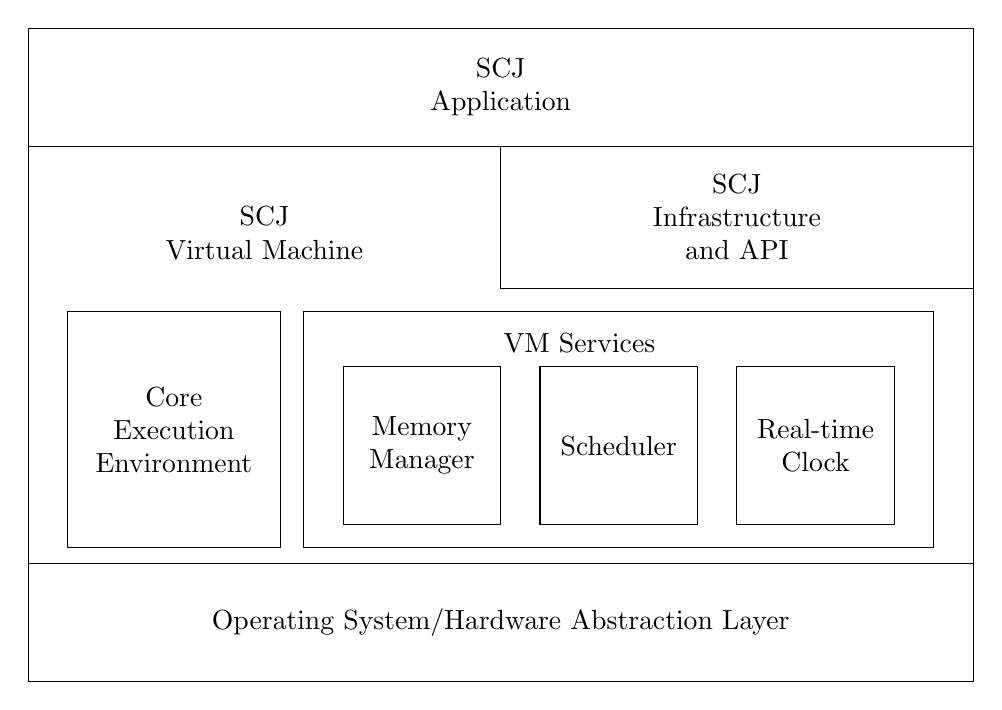
\begin{tikzpicture}
    \draw (0cm,0cm) rectangle (12cm,5.3cm);
    
    \draw (0.5cm,0.2cm) rectangle (3.2cm,3.2cm); \draw (3.5cm,0.2cm) rectangle
    (11.5cm,3.2cm); 
    \foreach \x in {1,...,3} \draw (\x * 2.5cm + 1.5cm,0.5cm)
    rectangle (\x * 2.5cm + 3.5cm,2.5cm) coordinate[pos=0.5](VMService\x);
    
    \node[align=center] at (3cm,4.2cm) {SCJ\\Virtual Machine};
    \node[align=center] at (1.85cm,1.7cm) {Core\\Execution\\Environment};
    \node[align=center] at (7cm,2.8cm) {VM Services}; 
    \node[align=center] at (VMService1) {Memory\\Manager};
    \node[align=center] at (VMService2) {Scheduler};
    \node[align=center] at (VMService3) {Real-time\\Clock};
    
    \draw (0cm,5.3cm) rectangle (12cm,6.8cm) node[pos=0.5,align=center]
    {SCJ\\Application}; \draw (6cm,3.5cm) rectangle (12cm,5.3cm)
    node[pos=0.5,align=center] {SCJ\\Infrastructure\\and API};
    
    \draw (0cm,-1.5cm) rectangle (12cm,0cm) node[pos=0.5,align=center]
    {Operating System/Hardware Abstraction Layer};
  \end{tikzpicture}
  \caption{A diagram showing the structure of the SCJ virtual machine and its
    relation to the SCJ infrastructure and the operating system/hardware
    abstraction layer.}
  \label{scjvm-fig}
\end{figure}

The core execution environment is not necessarily required to use any particular
means to run the bytecode.  It may interpret bytecode instructions, just-in-time
compile the bytecode, or execute native code precompiled from Java bytecode (and 
in such a case the compiler is regarded as part of the core execution
environment).  As we have already seen, many existing SCJVMs adopt the approach 
of compiling to native code, and so our specification of the core execution 
environment will focus on the construction of a compilation strategy, which is
discussed in the next section.

The compiled code in the core execution environment will need to call additional
functions to handle certain features of SCJ.  For example, as alluded to above,
the code to handle the \texttt{new} instruction must ensure the allocation is
performed withing the correct allocation context.  Some of these functions are
also required for implementing the SCJ libraries.  So it is sensible to
implement them alongside the core execution environment in what we have called
the virtual machine services.

The requirements for the virtual machine services are identified from
requirements imposed by the SCJ specification, with some consideration given to
the approaches taken by existing SCJVMs where the specification is unclear.  As
can be seen from Figure~\ref{scjvm-fig}, we group the virtual machine services
into three areas:
\begin{itemize}
\item the memory manager, which manages backing stores for memory areas and
  allocation within them;
\item the scheduler, which manages threads and interrupts, and allows for
  implementation of SCJ event handlers; and
\item the real-time clock, which provides an interface to the system real-time
  clock.
\end{itemize}
Each of these services is used either by the core execution environment or by
the SCJ infrastructure; some of the services also rely on each other.  For
example, the scheduler must update the allocation context in the memory manager
when performing a thread switch.

The virtual machine services may make use of low-level operating system
services to access hardware.  These operating system services may be supplied by
a full-featured operating system on which the virtual machine runs or may simply
be a minimal set of services required to run the virtual machine.  The latter
case is desirable for low-end embedded systems that lack the resources to
run a general operating system.  In our research, we need to identify the SCJVM
requirements.  As indicated previously, there is currently no accepted set of
such requirements.  We need them as part of the target machine for compilation
of SCJ programs.

\section{Compilation Strategy}

% change to present tense in the thesis
For the core execution environment, we will adopt the approach of
compilation from Java bytecode to C. The reason for the choice of C as
a target language is the same as that of other SCJ virtual machines,
particularly the icecap HVM: C is a language already widely used in
the area of embedded systems and is sufficiently lightweight to permit
its use as a compilation target.

As already mentioned, we intend adopt the algebraic approach in order to show
that the compilation is correct.  This will involve defining the semantics of
Java bytecode and C in terms of the specification language \Circus{}.  There is
much existing work on the formal semantics of Java bytecode~\cite{bertelsen2000,
  jones1998, stark2001, alves1999a, bogdanas2015, lochbihler2012a} and
C~\cite{campbell2012, ellison2012, krebbers2014} that can be used to aid in
that.

We expect that the semantics of Java bytecode for an SCJVM will be similar to
that of standard Java bytecode, except that the \texttt{invokedynamic}
instruction will be absent, since SCJ does not allow dynamic class loading.
Moreover, instructions such as \texttt{new} will have to be aware of the SCJ
memory and scheduling models.

When the semantics of Java bytecode and C are defined, we will define and prove
the refinement rules that specify the compilation.

\section{Formal Model}

In addition to the formal models of Java bytecode and C that are required for
specifying the compilation, a formal model of the virtual machine services is
also required.  The model will allow the requirements to be stated more
precisely and their consistency checked.  We will model the virtual machine
services in \Circus{} for ease of composition with the core execution
environment.  Formal models of requirements, Java bytecode and C are needed as
part of the characterisation of the normal form to be targetted in the algebraic
compilation approach. 

\section{Proofs}

It must be shown that the formal model of the virtual machine services is
consistent and that all the error cases have been accounted for.  The refinement
rules for the compilation will also require proofs.  These proofs will be
constructed from the basic laws of \Circus{}, which come from the UTP semantics
of \Circus{}~\cite{oliveira2009}.

\section{Mechanisation}

In order to ensure no mistakes are made during the proof, it should be
mechanised using an automated theorem prover. This provides assurance that the
proof is correct and can also make testing of the model easier due to the
code-generation facilities of theorem provers.  We will use Isabelle as our theorem
prover with its existing implementations of \Circus{}~\cite{feliachi2012} and 
the UTP~\cite{foster2015}.  The small axiomatic core of Isabelle helps to ensure
that theories implemented in it are correct, giving greater certainty that
proofs using them are sound.

\section{Final Considerations}

We already have some preliminary results identifying the requirements for
virtual machine services and constructing a formal model of them, which are
presented in the next chapter.  The formal model should have a machine-checked
proof of consistency but that remains to be completed.  We have not yet
specified the core execution environment.  The work presented in the next
chapter has also been submitted to the Java Technologies for Real-time and
Embedded Systems conference~\cite{baxter2015submitted}.  Our work is also
related to some work verifying the icecap HVM scheduler and we have contributed
to a paper on that, which is in preparation~\cite{freitas2015inpreparation}.

\chapter{Requirements of a Safety-Critical Java Virtual Machine}
\label{requirements-chapter}

We present here our preliminary work specifying the requirements for the
services of an SCJVM.  We specify the requirements for each of the virtual
machine services separately: the memory manager in
Section~\ref{memory-manager-section}, the scheduler in
Section~\ref{scheduler-section}, and the real-time clock in
Section~\ref{realtime-clock-section}.  Finally, we present an overview of the
formal model of the virtual machine services in
Section~\ref{formal-model-section}.

\section{Memory Manager API}
\label{memory-manager-section}

The SCJVM memory manager deals with the raw blocks of memory used as backing
stores for the memory areas of SCJ. The memory areas themselves are Java objects
and so are dealt with by the core execution environment and accessed through the
SCJ API. Backing stores here are assumed to have unique identifiers that can be
used to refer to them, these identifiers could simply be pointers to the
physical blocks of memory used for backing stores.

There is initially one backing store, called the root backing store, that has
its size set when the SCJVM starts up to cover all the memory available for
allocation in backing stores. We do not allow the root backing store to be
resized or destroyed so that there is always a fixed base for the layout of 
memory. The root backing store could be used as the backing store for the
immortal memory area. A backing store may have other backing stores nested
within it so that a possible memory layout is as shown in 
Figure~\ref{memory-fig}, with the backing store of mission memory nested within
the root backing store and the backing stores for the per-release memory of each
schedulable object in a mission nested within the mission memory's backing
store.

\begin{figure}[ht]
  \centering
  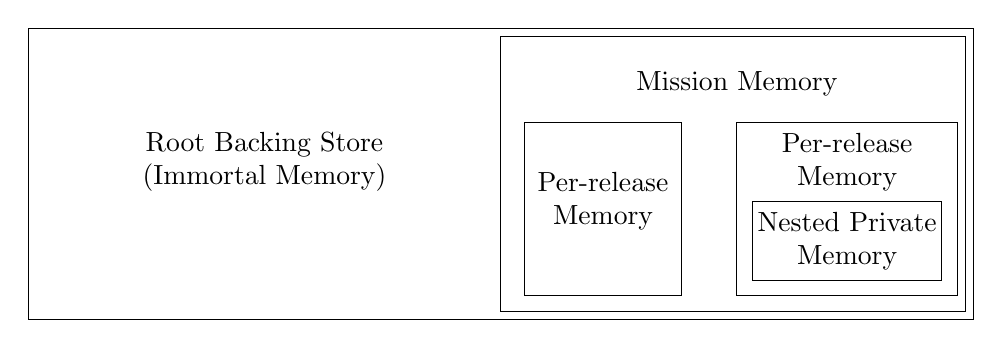
\begin{tikzpicture}
    \draw (0,0) rectangle (12,3.7);
    \node[align=center] at (3,2) {Root Backing Store\\(Immortal Memory)};
    
    \draw (6,0.1) rectangle (11.9,3.6);
    \node[align=center] at (9,3) {Mission Memory};
    
    \draw (6.3,0.3) rectangle (8.3,2.5);
    \node[align=center] at (7.3,1.5) {Per-release\\Memory};
    
    \draw (9,0.3) rectangle (11.8,2.5);
    \node[align=center] at (10.4,2) {Per-release\\Memory};
    
    \draw (9.2,0.5) rectangle (11.6,1.5);
    \node[align=center] at (10.4,1) {Nested Private\\Memory};
  \end{tikzpicture}
  \caption{An illustration of an example memory layout}
  \label{memory-fig}
\end{figure}

The operations of the memory manager API are summarised in
Table~\ref{memory-manager-table}. In addition to the inputs and outputs
described there, there should also be some system of reporting erroneous inputs,
whether that be exceptions, global error flags or particular return values
signalling errors. The conditions that cause an error to be reported are listed
in the final column of the table.

\begin{table}[ht]
  \centering
  \footnotesize
  \begin{tabular}{|l|p{3cm}|p{3cm}|p{3.6cm}|}
    Operation & Inputs & Outputs & Error Conditions \\
    \hline
    getRootBackingStore &
      (none) &
      backing store identifier &
      (none)
    \\getCurrentAllocationContext &
      (none) &
      backing store identifier &
      (none)
    \\setCurrentAllocationContext &
      backing store identifier &
      (none) &
      invalid identifier
    \\getTotalSize &
      backing store identifier &
      size in bytes &
      invalid identifier
    \\getUsedSize &
      backing store identifier &
      size in bytes &
      invalid identifier
    \\getFreeSize &
      backing store identifier &
      size in bytes &
      invalid identifier
    \\findBackingStore &
      memory pointer &
      backing store identifier &
      no backing store found
    \\allocateMemory &
      size in bytes &
      memory pointer &
      insufficient free memory
    \\makeBackingStore &
      size in bytes & 
      backing store identifier &
      insufficient free memory
    \\clearCurrentAllocationContext &
      (none) &
      (none) &
      nested backing store in use
    \\resizeBackingStore &
      backing store identifier \newline
      size in bytes &
      (none) &
      invalid identifier \newline
      insufficient free space \newline
      backing store is root \newline
      backing store not empty \newline
      backing store not only child
    \\createStack &
      size in bytes &
      stack identifier &
      insufficient free space
    \\destroyStack &
      stack identifier &
      (none) &
      invalid identifier
  \end{tabular}
  \caption{The operations of the SCJVM memory manager}
  \label{memory-manager-table}
\end{table}

The root backing store described above is always available to the SCJ
infrastructure through the \texttt{get\-Root\-Backing\-Store} operation. An SCJ
program does not have direct access to the root backing store except through
memory areas provided by the infrastructure.

In addition to managing the layout of backing stores in general, the memory
manager must also track what the current allocation context is. The operations
\texttt{get\-Cur\-rent\-Allo\-cation\-Con\-text} and
\texttt{set\-Cur\-rent\-Allo\-cation\-Con\-text} provide a means to get and set the
current allocation context. The functionality of changing the allocation context
is used by the methods of the SCJ API that allow code to be run with a different
memory area as allocation context, such as \texttt{execute\-In\-Area\-Of()} and
\texttt{enter\-Private\-Memory()}. The memory manager stores each thread's
allocation context and queries the scheduler as to which thread is current when
it performs operations affecting the current allocation context.

It is possible to obtain information about the used and available space in a given
backing store using the operations \texttt{get\-Total\-Size},
\texttt{get\-Used\-Size}, and \texttt{get\-Free\-Size}. This information is made
available to SCJ programs through the interface provided by memory areas.

Another query that can be made concerning backing stores is that of which
backing store a particular memory address lies in. This information can be
obtained by the \texttt{find\-Backing\-Store} operation and is required by the
infrastructure for obtaining the memory area of a given object.

Allocation within backing stores is possible through the
\texttt{allo\-cate\-Memory} operation, which allocates blocks of memory within
the current allocation context. This operation is provided in order for the core
execution environment to implement the \texttt{new} bytecode instruction and
should not be directly available to the program or infrastructure. Allocations
within backing stores must not cause fragmentation, so as to fulfil real-time
predictability requirements. The operation \texttt{allo\-cate\-Memory} must also
zero the memory it allocates, in order to properly match the semantics of
\texttt{new}.
 
Allocation of backing stores, which may require additional information attached
to them, is provided for by \texttt{make\-Back\-ing\-Store}, which is available
to the infrastructure for use when creating new memory areas. A new backing
store is created nested within the current allocation context. The
infrastructure is responsible for storing the backing store identifier returned
by the \texttt{make\-Backing\-Store} operation. The allocation of backing stores
is required to be done in constant time without fragmentation.

Deallocation of memory in backing stores cannot be done directly as that could
introduce fragmentation and would defeat the scoped memory model of
SCJ. Instead, the SCJVM provides for clearing a backing store when the memory
area it serves is no longer in use. This functionality is provided by the
operation \texttt{clear\-Current\-Allocation\-Context}, which clears the current
allocation context. It is not necessary to track exactly which object are
deallocated by this operation as SCJ does not have object finalisers. The
clearing of a backing store includes the clearing and removal of all backing
stores nested within it. This would create a problem if the parent backing store
is cleared while another thread is using a backing store within it as an
allocation context. However, such a situation should not occur as the backing
stores of mission memory and immortal memory are the only backing stores that
contain backing stores in use by different threads. Mission memory is only
cleared when all the event handler threads within the mission have finished and
immortal memory should never be cleared.

The last operation on backing stores is their resizing. This is provided for by
\texttt{resize\-Backing\-Store} but, as resizing a backing store presents a lot
of difficulties in terms of fragmentation, there are several restrictions. In
addition to being a valid backing store and there being enough space in the
parent backing store for the resizing to take place, a backing store to be
resized must not be the root backing store and must be empty and the only
backing store within its parent.  However, the only situations in which a
backing store resize is required are resizing of mission memory in between
missions and resizing of nested private memory when it is reentered. In both
these cases all the above points hold.

In addition to managing backing stores, the memory manager must also manage
stacks, which are placed in a separate area of memory to the backing stores. The
operations \texttt{create\-Stack} and \texttt{destroy\-Stack} allow for stacks
to be created and destroyed respectively. The stack space must not be fragmented
but this should not be an issue as stacks for threads are allocated together
when the mission is initialised and destroyed together when the mission
ends. That remains true at level 2 where nested missions are permitted as the
nested mission's stacks will be allocated after the stacks of it's parent
mission and will be destroyed before the parent mission ends. Like backing
stores, stacks are referred to by unique identifiers that may simply be pointers
to the space allocated for the stack.

\section{Scheduler API}
\label{scheduler-section}

The SCJVM scheduler manages the scheduling of threads. The operations of the
scheduler are summarised in Table~\ref{scheduler-table}.

\begin{table}[ht]
  \centering
  \footnotesize
  \begin{tabular}{|l|p{3cm}|p{2.2cm}|p{2.7cm}|}
    Operation & Inputs & Outputs & Error Conditions \\
    \hline
    getMaxSoftwarePriority &
      (none) &
      priority level &
      (none)
    \\getMinSoftwarePriority &
      (none) &
      priority level &
      (none)
    \\getNormSoftwarePriority &
      (none) &
      priority level &
      (none)
    \\getMaxHardwarePriority &
      (none) &
      priority level &
      (none)
    \\getMinHardwarePriority &
      (none) &
      priority level &
      (none)
    \\getMainThread &
      (none) &
      thread identifier &
      (none)
    \\makeThread &
      entry point \newline
      priority level \newline
      backing store identifier \newline
      stack identifier &
      thread identifier &
      invalid priority \newline
      invalid backing store \newline
      invalid stack
    \\startThread &
      thread identifier &
      (none) &
      invalid identifier
    \\getCurrentThread &
      (none) &
      thread identifier &
      (none)
    \\destroyThread &
      thread identifier &
      (none) &
      invalid identifier
    \\suspendThread &
      (none) &
      (none) &
      (none)
    \\resumeThread &
      thread identifier &
      (none) &
      invalid identifier
    \\setPriorityCeiling &
      pointer to object \newline
      priority level &
      (none) &
      invalid priority
    \\takeLock &
      pointer to object &
      (none) &
      lock in use
    \\releaseLock &
      pointer to object &
      (none) &
      lock not held
    \\attachInterruptHandler &
      interrupt identifier \newline
      entry point &
      (none) &
      invalid interrupt
    \\detachInterruptHandler &
      interrupt identifier &
      (none) &
      invalid interrupt
    \\getInterruptPriority &
      interrupt identifier &
      priority level &
      invalid interrupt
    \\disableInterrupts &
      (none) &
      (none) &
      (none)
    \\enableInterrupts &
      (none) &
      (none) &
      (none)
  \end{tabular}
  \caption{The operations of the SCJVM scheduler}
  \label{scheduler-table}
\end{table}

Each thread is scheduled according to a priority level. The SCJ standard
requires that there be at least 28 priorities and separates them into hardware
and software priorities, with hardware priorities being higher than software
priorities. The range of priorities that a VM actually supports may vary between
different VM implementations within these restrictions. To allow the range of
supported priorities to be determined and support corresponding methods in the
SCJ API, the minimum and maximum hardware and software priority levels can be
obtained with \texttt{get\-Max\-Soft\-ware\-Pri\-or\-ity},
\texttt{get\-Min\-Soft\-ware\-Pri\-or\-ity},
\texttt{get\-Max\-Hard\-ware\-Pri\-or\-ity}, and
\texttt{get\-Min\-Hard\-ware\-Pri\-or\-ity}. The SCJVM chooses a default normal
software priority for threads, that can be queried through the
\texttt{get\-Norm\-Soft\-ware\-Pri\-or\-ity} operation.

Initially there is one thread running, which is called the main thread. The main
thread is created when the VM starts and has an implementation-defined
priority. The main thread can be suspended by the infrastructure when it is not
needed and resumed when it is needed again, using the operations mentioned
below. This allows it to be used for setting up the SCJ application and
missions, then suspended during mission execution. The main thread's identifier
can be retrieved using the \texttt{get\-Main\-Thread} operation.

Threads other than the main thread can be created by the \texttt{create\-Thread}
operation, which takes the entry point and priority level of the thread to be
created, as well as a backing store as the allocation context and a stack to use
for the thread. This operation returns the identifier of the newly created
thread, which must be stored by the infrastructure. The SCJVM does not
distinguish between the different thread release conditions so for
periodic and one-shot threads the infrastructure must set a timer separately
using the real-time clock API when a thread is created. The only priorities
allowed for threads are the software priorities, as hardware priorities are
reserved for interrupts. The backing store supplied here is only used to set the
backing store in the memory manager when the thread starts and is not stored by
the scheduler beyond that.

The SCJVM threads that are eligible to run must be scheduled as if they are
placed in queues with one queue for each priority. At each moment in time, the
thread at the front of the highest priority non-empty queue is running. A thread
becomes eligible to run after it is started and stops being eligible to run when
it is blocked. A thread is started using the \texttt{start\-Thread} operation
and must be started by the infrastructure when its enclosing mission starts. The
reason for the separation between thread creation and thread starting is to
ensure that threads all start together after mission initialisation has been
completely finished.

The identifier of the currently running thread can be obtained through the
\texttt{get\-Current\-Thread} operation. This operation may be used by the
infrastructure as part of obtaining the current schedulable object but is mainly
intended for use by the memory manager in order to discern what the current
allocation context is.

A thread can be suspended, causing it to become blocked, and resumed, causing it
to become eligible to run again, by the operations \texttt{suspend\-Thread} and
\texttt{resume\-Thread}. These operations are only visible to the program
through \texttt{wait()} and \texttt{notify()} at level 2. These operations are
also used in hardware communication, when a thread must wait for hardware to
complete a request, and to implement thread release, whereby a thread
remains suspended until released.

A thread that has been created can then be destroyed with the
\texttt{destroy\-Thread} operation, which removes the thread from the scheduler.
Destroying a thread does not automatically destroy its stack or the backing
store being used as its allocation context. The SCJ infrastructure should not
destroy a thread while it is running as a thread should only be destroyed when
the mission it is part of is ending. The infrastructure should instead ensure
that all threads in a mission are suspended before destroying them.

The SCJVM must support priority ceiling emulation, as it is required by
SCJ. This is handled by providing the \texttt{set\-Priority\-Ceiling} operation
that associates a priority ceiling value to an object identified by a
pointer. An object that does not have its priority ceiling explicitly set has a
priority ceiling equal to the default ceiling, which should be the highest
software priority but it is possible that a virtual machine could have an option
to change the default priority ceiling. Note that the SCJVM scheduler does not
require a notion of object in order to associate priority ceilings to objects as
the object's pointer can be used as an opaque identifier.

The operations for taking and releasing locks are \texttt{takeLock} and
\texttt{releaseLock}. A thread can only take a lock if its active priority and
the ceiling priorities of any other objects it holds the locks for is less than
or equal to the ceiling priority of the object the lock is being taken on. Only
one thread can take a given object's lock at a time. When a lock is taken, the
thread's active priority is raised to the object's priority ceiling. When a
thread releases a lock, the thread's active priority is lowered to its previous
active priority (the thread may hold nested locks on multiple objects).

The SCJVM scheduler must also manage interrupts, as interrupt handlers have
priorities (though these should be in the hardware priority range) and so must
be dealt with within the priority scheduling model. An interrupt handler can be
attached to a given interrupt using the \texttt{attach\-Interrupt\-Handler}
operation and an interrupt's handler can be removed with the
\texttt{detach\-Interrupt\-Handler} operation. An interrupt with no handler
attached to it is ignored. The clock interrupt coming from hardware is handled
by the SCJVM clock (see Section~\ref{realtime-clock-section}) and converted into
a clock interrupt that is passed to the scheduler for handling by the attached
interrupt handler (which should simply call the \texttt{triggerAlarm()} method
of \texttt{Clock}).

Each interrupt has a priority associated with it, which is set by the SCJVM on
startup and cannot be changed by the application. These interrupt priorities
must be hardware priorities. An interrupt handler will interrupt any
lower-priority interrupt handler and any running threads, and blocks
lower-priority interrupt handlers from running until it has finished. The
priority associated with each interrupt can be obtained by the
\texttt{get\-Interrupt\-Priority} operation.

Interrupts can be disabled using the \texttt{disable\-Interrupts} operation and
re-enabled using the \texttt{enable\-Interrupts} operation. While interrupts are
disabled no interrupt handlers can run but it is implementation-defined as to
whether or not interrupts fired while interrupts are disabled are lost.

\section{Real-time Clock API}
\label{realtime-clock-section}

The SCJVM must manage the system real-time clock, providing an interface that
allows for the time to be read and alarms to be set to trigger time-based
events. The operations of the SCJVM real-time clock are summarised in
Table~\ref{realtime-clock-table}.

\begin{table}[ht]
  \centering
  \footnotesize
  \begin{tabular}{|l|p{0.9cm}|p{1.8cm}|p{2.3cm}|}
    Operation & Inputs & Outputs & Error Conditions \\
    \hline
    getSystemTime &
      (none) &
      time &
      (none)
    \\getSystemTimePrecision &
      (none) &
      time precision &
      (none)
    \\setAlarm &
      time &
      (none) &
      time in past
    \\clearAlarm &
      (none) &
      (none) &
      (none)
  \end{tabular}
  \caption{The operations of the SCJVM real-time clock}
  \label{realtime-clock-table}
\end{table}

The main function of the real-time clock API is to provide access to the system
time through the \texttt{get\-System\-Time} operation. The SCJ API deals with
time values in terms of milliseconds-nanoseconds pairs, that should also be the
format for time values passed to and from the SCJVM though another format could
be used. The system time may be measured from January 1, 1970 or from the system
start time (in case there is no reliable means of determining the date
and time), and so may not correspond to wall-clock time.

The time between ticks of the system clock (its precision) must be made
available through the \texttt{get\-System\-Time\-Precision} operation. The
clock's precision must not change.

The SCJVM must also provide a facility to set an alarm that sends a clock
interrupt to the scheduler when a specific time is reached. This facility is
provided by the \texttt{set\-Alarm} function, which accepts an absolute time
value at which the alarm should trigger. The time passed to \texttt{set\-Alarm}
is required to not be in the past. Running code at a specified relative time
offset should be handled by the infrastructure. Once a alarm has triggered, it
is removed and a new alarm must be set in order to perform events periodically.

The current alarm (if any) can be cleared using the \texttt{clear\-Alarm}
operation.

\section{Formal Model}
\label{formal-model-section}

The formal model of the SCJVM is written in the \Circus{} specification
language~\cite{oliveira2009} In this section, we present an overview of our
model. We then present part of the memory manager model to to show how it is
constructed. The complete model can be found in~\cite{baxter2015}. It is type
checked with Community Z Tools and we have started to prove some basic
properties of the memory manager using Z/Eves.

In our model, each of the components of the SCJVM shown in
Figure~\ref{scjvm-fig} is specified by a single process whose channels represent
the services they provide.  The whole collection of VM services are then
specified by a parallel composition of the memory manager, scheduler and clock
processes. In this case, parallelism is being used to define a conjunction of
requirements. 

The processes synchronise on the channels they share, specified in the
sets $MMSInterface$ and $RTCSInterface$. The set $MMSInterface$ is the interface
between the memory manager and the scheduler, which contains a channel to get
the current thread from the scheduler, and channels to inform the memory manager
of the creation and destruction of threads. The interface between the real-time
clock and the scheduler, $RTCSInterface$, contains a channel to pass the clock
interrupt to the scheduler for handling. The channels used for internal
communication between the VM services are hidden so that the only channels that
can be used to communicate with the VM services are those used to represent the
services in Tables~\ref{memory-manager-table}, \ref{scheduler-table} and
\ref{realtime-clock-table}, and those used for communication with the core
execution environment.
%
\begin{circus}
  VMServices \circdef \\
  \t1 ((MemoryManager \lpar MMSInterface \rpar Scheduler) \\
  \t2 \lpar RTCSInterface \rpar RealtimeClock) \circhide VMServicesInternals
\end{circus}
%
The parallel composition of $VMServices$ with a process representing the core
execution environment (which, as mentioned, we do not specify here)
specifies the full SCJVM.

Our model of the scheduler is similar to other formal models of priority
schedulers~\cite{ferreira2014, gotsman2013, klein2014, lime2009}, and the
real-time clock specification is fairly simple and just manages the current time
and any alarm that may be set. For those reasons, we do not go into detail on
the scheduler on clock models here. Instead, we present part of the memory
manager model, which is the most complex of the three VM services.  We show the
memory manager state and some of the operations. We also explain how the formal
specification reflects the requirements identified in
Section~\ref{memory-manager-section}.

The memory manager specification begins by declaring a type, $MemoryAddress$, of
memory addresses to be the set of natural numbers.  This then allows for
specification of a type, $ContiguousMemory$, that contains contiguous ranges of
memory addresses and is used to specify that backing stores must not be
fragmented.
%
\begin{zed}
  MemoryAddress == \nat \\
  ContiguousMemory == 
  \{~ m : \power MemoryAddress | \exists a, b : MemoryAddress @ m = a \upto b ~\}
\end{zed}
%
Backing stores are identified by identifiers that are elements of a type
$BackingStoreID$. These are simply opaque identifiers and there are no
constraints on $BackingStoreID$ beyond the fact that it exists.

We specify backing stores in two parts. The first part, $MemoryBlock$, stores
the used, free and total memory and allows for allocation within it. This aspect
of backing stores is separated out because it is also used in specifying the
stack space, since allocation of memory also occurs there.The variables $used$
and $free$ correspond to the areas of used and free memory, while $total$
represents the whole memory area covered by the $MemoryBlock$. Note that $free$
and $total$ are required to be contiguous to enforce the requirement that there
must be no fragmentation whereas it is not necessary that $used$ is simply
specified to be a set of memory addresses. There are two invariants on
$MemoryBlock$, identified by the predicates in the schema above. The first
invariant simply specifies that $used$ and $free$ must be contained in $total$,
but it does not require them to cover $total$ as there may be some additional
memory overhead. The second invariant requires $used$ and $free$ to be disjoint.
%
\begin{schema}{MemoryBlock}
  free, total : ContiguousMemory \\
  used : \power MemoryAddress \\
\where
  used \cup free \subseteq total \\
  used \cap free = \emptyset \\
\end{schema}
%
A $MemoryBlock$ is initialised by the $MemoryBlockInit$ operation, which accepts
as an input a contiguous area of memory, $addresses?$, that it should cover. The
final state of the operation is represented by variables obtained by placing a
prime on the names of the state components. The variable $total'$ is specified
to be equal to $addresses?$ and $used'$ is specified to be empty. The variable
$free'$ is permitted to take any value, provided that it is a subset of
$addresses?$.
%
\begin{schema}{MemoryBlockInit}
  MemoryBlock~' \\
  addresses? : ContiguousMemory \\
\where
  total' = addresses? \\
  free' \subseteq addresses? \\
  used' = \emptyset \\
\end{schema}
%
As an example of an operation on $MemoryBlock$, we present $MBAllocate$, the
operation of allocating memory within a $MemoryBlock$. This operation takes an
input $size?$ that is the requested size of the allocated memory, and outputs an
area of contiguous memory called $allocated!$. There is a precondition on this
operation that $size?$ must be smaller than the size of $free$, to ensure that
there is enough free space to fulfil the allocation request. The output,
$allocated!$, is then specified to be of the requested size and contained within
$free$. The final state $used'$ is obtained by adding $allocated!$ to $used$ and
$free'$ is obtained by removing $allocated!$ from $free$. Finally, it is
specified that $total$ does not change.
%
\begin{schema}{MBAllocate}
  \Delta MemoryBlock \\
  size? : \nat \\
  allocated! : ContiguousMemory
\where
  size? \leq \# free \\
  \# allocated! = size? \land allocated! \subseteq free \\
  used' = used \cup allocated! \\
  free' = free \setminus allocated! \\
  total' = total \\
\end{schema}
%
With $MemoryBlock$ specified, the remaining parts of the backing store state are
added in the schema $BackingStore$, which is a $MemoryBlock$ with a variable,
$self$, to store its own identifier and a finite set, $children$, of the
identifiers of its immediate children. The invariants specify that it cannot be
a child of itself and that the overhead, left loosely specified in
$MemoryBlock$, must have a size equal to some constant
$backingStoreOverhead$. The invariants inherited from $MemoryBlock$ are also
required to hold.
%
\begin{schema}{BackingStore}
  MemoryBlock \\
  self : BackingStoreID \\
  children : \finset BackingStoreID \\
\where
  self \notin children \\
  \# total = \# used + \# free + backingStoreOverhead
\end{schema}
%
Initialisation of a $BackingStore$ is handled by the operation
$BackingStoreInit$, which behaves as $MemoryBlockInit$ with the additional
precondition that the size $addresses?$ must be larger than
$backingStoreOverhead$ and the requirement that $free'$ be made smaller than
$addresses?$ to allow space for $backingStoreOverhead$. For the new state
components, $self'$ is specified by an additional input $newID?$ and $children'$
is specified to be empty.
\begin{schema}{BackingStoreInit}
  BackingStore~' \\
  MemoryBlockInit \\
  newID? : BackingStoreID \\
\where
  \# addresses? \geq backingStoreOverhead \\
  \# free' = \# addresses? - backingStoreOverhead \\
  self' = newID? \\
  children' = \emptyset \\
\end{schema}
%
An example of a $BackingStore$ operation is allocating space for a new child
backing store within its parent. That operation is given by the schema
$BSAllocateChild$ below.
%
\begin{schema}{BSAllocateChild}
  \Delta BackingStore \\
  MBAllocate \\
  childID! : BackingStoreID \\
  \where
  childID! \notin children \land childID! \neq self \\
  children' = children \cup \{ childID! \} \\
  self' = self
\end{schema}
%
This operation is based on $MBAllocate$, but it has an additional output,
$childID!$, which is the identifier of the newly allocated child, and it
specifies how the extra state components in $BackingStore$ are updated. The new
child's identifer is specified to not be the identifier of an existing child and
must not be the identifier of the backing store itself. The final state
$children'$ is specified to add $childID!$ to $children$ and $self$ does not
change. This operation is made into a robust operation, $RBSAllocateChild$, that
handles the case where the precondition does not hold by outputting a value
$report!$, which is either a reported error or the value $okay$.

Backing stores are managed by the global memory manager, the state of which is
given by the schema below. The global memory manager state contains a partial
function, $stores$, that relates backing store identifiers to the backing
stores, along with the identifier, $rootBackingStore$, of the root backing store
and a relation, $childRelation$ between backing store identifiers and the
identifiers of their direct children. The global state also contains a map,
$threadACs$, from thread identifiers to their allocation context, which is used,
together with information obtained from the scheduler, to perform operations on
the current allocation context.

The relationships between the backing stores are specified by the invariants of
this state as defined by the predicates in the schema above. The first invariant
specifies that the root backing store must be a valid identifier (this is
implied by the sixth invariant but is written separately for clarity). The
second invariant is an injectivity condition on $stores$, requiring that no two
backing stores have the same identifier. The third invariant requires that a
backing store's children are all disjoint and contained in that backing store's 
used memory. The fourth invariant requires that
the thread allocation contexts be valid backing stores. The fifth invariant 
defines $childRelation$, using the set of children in the backing store record
to form a relation between backing store identifiers. The sixth invariant uses
the reflexive transitive closure of $childRelation$ to specify that every known
backing store must be a (direct or indirect) child of the root backing store or
the root backing store itself. Lastly, the seventh invariant specifies that no
backing store can be a (direct or indirect) child of itself.
%
\begin{schema}{GlobalMemoryManager}
  stores : BackingStoreID \pfun BackingStore \\
  childRelation : \\
    \t1 BackingStoreID \rel BackingStoreID \\
  rootBackingStore : BackingStoreID \\
  threadACs : ThreadID \pfun BackingStoreID \\
\where
  rootBackingStore \in \dom~stores \\
  \forall b: \dom~stores @ (stores~b).self = b \\
  \forall b : \ran stores @ \exists m : \power b.used @ 
    (\lambda x : b.children @ (stores~x).total)~\partition~m \\
  \ran threadACs \subseteq \dom stores \\
  childRelation = \bigcup \{ i : \dom~stores @ \{ j : (stores~i).children @ (i,j) \} \} \\
  \dom stores = (childRelation\star) \limg \{ rootBackingStore \} \rimg \\
  \forall s : \dom stores @ s \notin childRelation\plus \limg \{ s \} \rimg \\
\end{schema}
%
The operations on the memory manager are specified using the Z idiom of
promotion, which allows operations on a local state to be lifted to operations on
a global state.  This allows simple operations on the backing store records to be
used to update the backing stores in the $stores$ function.  As an
example we present the $GlobalMakeBS$ schema that specifies the creation of a
backing store within another.

Much of this operation's complexity is due to the fact that it promotes two
operations: $RBSAllocateChild$ and $BackingStoreInit$. The allocation occurs in
the current allocation context, identified by the input $allocationContext?$. It
is determined by obtaining the current thread from the scheduler, looking up its
allocation context and passing it as an input to the operation specified by the
Z schema.  The operation produces as output the identifier $childID!$ of the
newly allocated backing store.

The first condition on the operation requires that the allocation context be a
valid backing store, that is, in the domain of $stores$. After that, the
existential quantifiers introduce variables local to the schema, specifying the
size of the allocated backing store, $actualSize$, to include some
implementation-defined overhead.

Then the promotions are specified, beginning with the operation
$RBSAllocateChild$. The variables $childID!$ and $childAddresses!$ are
identified with outputs of the promoted operation that have the same names. The
initial state for the promoted operation is taken from the backing store in
$stores$, and the final state is placed in the variable $parent$.  The output
$childID!$ is required to not be the identifier of another backing store. It is
required that no error be reported in the error reporting variable $report!$.

The second operation promoted is $BackingStoreInit$. The variables
$actualSize$, $childAddresses!$ and $childID!$ are passed to it as inputs via
renaming. The final state of the promoted operation is stored in $child$.  The final 
states of both backing stores, $parent$ and $child$ are stored in the $stores$
function, with $childID!$ being used as the identifier of $child$. The 
specification of the operation ends by stating that all other state variables
remain the same.
%
\begin{schema}{GlobalMakeBS}
  \Delta GlobalMemoryManager \\
  size? : \nat \\
  allocationContext? : BackingStoreID \\
  childID! : BackingStoreID \\
\where
  allocationContext? \in \dom stores \\
  \exists actualSize : \nat | actualSize = size? + backingStoreOverhead @ \\
  \exists allocated! : ContiguousMemory @ \\
  \exists parent, child : BackingStore @ \\
  \t1 (\exists \Delta BackingStore; report! : Report | RBSAllocateChild [ actualSize / size? ] @ \\
    \t2 \theta BackingStore = stores~allocationContext? \land \\
    \t2 parent = \theta BackingStore~' \land \\
    \t2 childID! \notin \dom stores \land \\
    \t2 report! = okay) \land \\
  \t1 (\exists BackingStore~'; report! : Report | BackingStoreInit [ allocated! / addresses? ] @ \\
    \t2 child = \theta BackingStore~') \land \\
  \t1 stores' = stores \oplus \{ allocationContext? \mapsto parent, childID! \mapsto child \} \\
  rootBackingStore' = rootBackingStore \\
  childRelation' = childRelation \\
  threadACs' = threadACs \\
\end{schema}
%
Other global memory manager operations are similarly specified using
promotion. Operations on stacks are specified separately, using a
specification based on $MemoryBlock$.

\section{Final Considerations}

The requirements and formal model presented in this chapter are an important
part of the plan presented in the previous chapter as they specify the services
required to support an SCJ program.  These requirements are also necessary to
support the core execution environment, which will be specified in future work,
and so they lay the foundation for our work.

The formal model presented in this chapter is yet to be proved correct but it
has already demonstrated its worth by enabling the requirements to be stated
more precisely.  This has meant that various issues have arisen during creation
of the formal model that were not apparent in the informal statement of
requirements.  Resolving the issues in the formal model has, in turn, made the
informal requirements more precise and better structured.  It may be that
further modifications will be required as proof of the model progresses.  This
shows one of the great benefits of formal methods: that errors can be detected
which may not be easily visible to the human eye.

% add a final considerations section noting lessons learned from the
% formalisation and how it contributes to the research proposal

\chapter{Conclusions}
\label{conclusions-chapter}

% three sections: summary of contributions, related work, and future work
In this chapter we conclude by summarising the contributions of this
dissertation in Section~\ref{summary-section}.  We then discuss some related
work in Section~\ref{related-work-section}, providing the context for our work,
and the direction of future work in Section~\ref{future-work-section}.

\section{Summary of Contributions}
\label{summary-section}

In this dissertation we have considered the safety-critical variant of Java and
some virtual machines designed to run programs written in it.  We have concluded
that none of the virtual machines is formally verified and that many of them
precompile programs to native code.  Given the need for a formally verified
virtual machine, we have stated our aim to specify a framework within which an
SCJ virtual machine can be verified

Having noted that SCJ virtual machines employ compilation, we have surveyed some
of the work on compiler correctness, particularly how it relates to Java
compilation, and seen there are two approaches: the commuting-diagram approach
and the algebraic approach.  We have decided to adopt the algebraic approach and
chosen \Circus{} as a specification language.

As some preliminary work in specifying an SCJ virtual machine, we have
identified the requirements of the virtual machine services required to support
SCJ programs.  We have also constructed a formal model of those requirements in
the \Circus{} specification language.
% need more reflection on the preliminary results, check the conclusions of the
% JTRES paper for material

\section{Related Work}
\label{related-work-section}

% include material on related work from the JTRES paper
Our work is done in the context of a wider effort to facilitate fully verified
Safety-Critical Java programs.  There has already been work on generating
correct SCJ programs from \Circus{} specifications~\cite{cavalcanti2011,
  cavalcanti2013} and formalisation of the SCJ memory
model~\cite{cavalcanti2011a}.  As discussed earlier, there has also been work on
correct compilation of Java (and SCJ) programs~\cite{klein2006, strecker2002,
  lochbihler2010, duran2005, stark2001}.  All these works allow for creation of
correct programs and the focus of our work is on the next stage of running those
programs.  As we are adopting the approach of compilation to C, it should also
be noted that there has been much work on verified C
compilation~\cite{leroy2009a, leroy2009b, leroy2012, leinenbach2005, blazy2006},
thus allowing for complete verification down to executable code.

\section{Future Work}
\label{future-work-section}

Our future work will involve proving the correctness of the formal model of the
virtual machine services and specifying the core execution environment.  As
already discussed, this will involve defining the semantics of Java bytecode and
C in terms of \Circus{} and proving refinement laws between them.  This will be
mechanised in the Isabelle proof assistant.
% write more summarising chapter 3

Beyond the scope of our work, possible future work could include the
verification of an SCJ virtual machine using our framework or even the creation
of a correct-by-construction virtual machine from our specification.  The option
of deriving a correct virtual machine from our specification may be more
desirable than verifying an existing one.  This is because virtual machines can
often be complex and therefore difficult to verify in a structured way.
Moreover, while the effort of proving a virtual machine correct may uncover
bugs, it may be a challenge to fix them.  Also, the virtual machine may not exactly
meet our specification, requiring restructuring to merely allow the proof effort
to begin.  On the other, the fact that \Circus{} allows for refinement means that a
correct virtual machine can be constructed from our model in a stepwise and modular
fashion, being shown to be correct at each stage of the process.  Facilitating such
work is the ultimate aim of our work, in order to provide for
the correct running of SCJ programs.

\raggedright
\printbibliography
\end{document}

%  LocalWords:  modularise certifiability verifiers mechanisations checkable
%  LocalWords:  aperiodically schedulability associativity nondeterministic CSP
%  LocalWords:  precompiled precompilation disjunction schemas instantiation
%  LocalWords:  nondeterministically boolean datatype SCJVM
